\documentclass[11pt,a4paper]{article}
\usepackage{fontspec}
\setmainfont{TeX Gyre Pagella}
\newfontfamily\headfont{Inter}[UprightFont=*-ExtraBold,BoldFont=*-ExtraBold,Extension=.otf,Path=/usr/share/fonts/opentype/inter/]
\usepackage[a4paper,margin=2.3cm]{geometry}
\usepackage{graphicx,booktabs,float,caption,array,xcolor,amsmath}
\usepackage[hidelinks]{hyperref}
\usepackage{titlesec}
\usepackage[round]{natbib}
\usepackage{setspace}
\setstretch{1.05}
\renewcommand{\topfraction}{0.9}
\renewcommand{\bottomfraction}{0.8}
\renewcommand{\textfraction}{0.1}
\renewcommand{\floatpagefraction}{0.75}
\setlength{\parindent}{0pt}
\setlength{\parskip}{0.55em}
\titleformat{\section}{\headfont\Large}{\thesection}{0.8em}{}
\titleformat{\subsection}{\headfont\large}{\thesubsection}{0.8em}{}
\captionsetup{font=small,labelfont=bf}
\urlstyle{same}
\hypersetup{pdftitle={By Road and by Sea: Fastest Travel Times from Rome in the Roman Empire},pdfauthor={Tristan Hotham}}

\begin{document}
\begin{center}
{\Large\bfseries By Road and by Sea\par}
\vspace{0.4em}
{\large Fastest travel times from Rome in the Roman Empire, with Itiner-e roads,\\Pleiades ports and Casson's sailing speeds\par}
\vspace{1.2em}
{\large Tristan Hotham\par}
\vspace{0.3em}
{\small Independent researcher\\
ORCID: 0000-0003-4931-9349\\
DOI: \detokenize{10.5281/zenodo.23863542}\par}
\vspace{0.8em}
2026
\end{center}

\begin{quote}
\small
\begin{center}\textbf{Abstract}\end{center}
A companion study modelled travel from Rome over the Itiner-e network of Roman roads and found journeys of months: 210 days on foot to Carthage, because the road goes round North Africa. Here I add the sea. 211 ancient ports from Pleiades and the ancient voyage reports are joined to the roads and to a grid of 29,351 sea cells of 15 km covering the Mediterranean, the Black Sea and the Atlantic coast to Britain. Sailing speeds come from Casson's (1951) collection of ancient voyages and are calibrated to his Table 1 of 57 estimated sailing times between named ports: 5.2 knots running before the wind, 3.7 where my sources name no prevailing wind, and 1.0 to 1.6 knots dead into it, all within the ranges Casson gives. The summer etesian winds blow from the north in the Aegean and from the north-west in the central and eastern Mediterranean. The calibrated model falls inside Casson's range for 25\% of the Table 1 passages and within a quarter of it for 63\%, with a median of 1.01 times his estimate; a slower version that uses his median speeds and fits the speed into the wind to his 53 to 73 days from Alexandria to Rome manages 21\% and 44\%, with a median of 1.38. I headline the calibrated model, which matches the outward voyages that a journey from Rome mostly involves, and keep the slower one as a sensitivity test; the calibrated model makes the long voyage home from the east too quick. In summer, with the sea, Carthage is 5.8 days from Rome, Alexandria 12, London 30 and Constantinople 17 (36 with the slower model). The share of the provinces' land within 30 days of Rome on foot rises from 3.9\% by road alone to 59\%.

\textbf{Keywords:} Roman Empire; travel time; sea routes; sailing speeds; etesian winds; Itiner-e; Pleiades; network analysis
\end{quote}

\section{Introduction}
The roman-roads study \citep{hotham2026} used the Itiner-e dataset \citep{itinere,desoto2025} to model journeys from Rome on foot, by cart and by courier over 299,171 km of road. It gave long answers: London 81 days, Alexandria 180 and Carthage 210. The obvious objection, made by many readers, is that Romans did not make such journeys by road. The Mediterranean was the empire's main artery, and the grain fleets, officials, armies and letters that crossed it did so by ship whenever the season allowed.

This paper adds the sea to the same road network with a model that is deliberately simple and fully stated: ports from an open gazetteer, sea lanes over open water, sailing speeds taken from Casson's collection of ancient voyage reports and calibrated to his own estimated sailing times \citep{casson1951}, and one pattern of summer winds. It asks how much closer the sea brought the provinces to Rome, which places gained most, and how well such a simple model reproduces Casson's estimates and the voyages that ancient writers recorded. An interactive version (\url{https://maps.tristanhotham.com/roman-travel-times/}) runs the same model in the browser from any start.

The question has been studied before. Stanford's ORBIS model \citep{orbis,scheidel2014,scheidel2015} combines roads, rivers and sea routes with monthly wind and wave conditions, two kinds of ship and many modes of road travel. I do not use or reproduce its numbers. The model here is narrower but transparent, and it sits on the far more detailed Itiner-e road network.

\section{Data}
\textbf{Roads.} Itiner-e static version 2024 \citep{itinere}: 14,769 sections joined at 10,315 junctions, with lengths and a slope-based passability value, treated exactly as in \citet{hotham2026}.

\textbf{Ports.} Every place in the Pleiades gazetteer \citep{pleiades} typed as a port, harbour or anchorage that has a location, and 76 further harbours named in the voyage reports, the grain trade and the fleet bases (Ostia, Puteoli, Massilia, Byzantium, Ephesus and others), located by their Pleiades record or, where Pleiades has no single record, by the Itiner-e junction of that name. A port is kept if it lies within 25 km of the sea grid and 15 km of a road junction: 211 ports, 135 of them typed as ports in Pleiades.

\textbf{Sailing speeds.} Casson's tables of voyages with favourable and unfavourable winds, giving for each the route, the distance in nautical miles, the days taken, the speed in knots and the ancient source \citep{casson1951}. I use the article as published in its LacusCurtius online edition. His summary is that ancient ships averaged 4 to 6 knots over open water with a favourable wind, 3 to 4 knots through islands or along coasts, and less than 2 to 2\textonehalf{} knots against the wind. His Table 1 gives estimated sailing times, as ranges of days, for 57 pairs of named ports, among them 10 to 13 days from Rome to Alexandria and 53 to 73 days back.

\textbf{Winds and season.} The English Wikipedia article on the etesians \citep{wikietesian} describes them as strong, dry north winds of the Aegean that blow from about mid-May to mid-September, northerly in the central Aegean and north-westerly in the southern Aegean and around Crete. Casson notes that in summer there was no direct sailing from Alexandria to Rome because the winds did not permit it. The article on mare clausum \citep{wikimare} records that the period from November to March was considered the most dangerous for navigation.

\textbf{Land.} Natural Earth \citep{naturalearth}; provinces of about AD 117 from the Digital Atlas of the Roman Empire \citep{dare}.

\section{Methods}
\subsection{The sea grid}
Open water is divided into 15 km cells in a Lambert azimuthal equal-area projection centred on the Mediterranean; a cell is sea if its centre is not on Natural Earth 50m land. The Red Sea, the Baltic and the far Atlantic are excluded. A ship moves from a cell to any of its 16 nearest neighbours (the eight adjacent cells and the eight knight's moves) if the straight line between them stays at sea. The Bosporus, Dardanelles, Kerch Strait and Strait of Messina, too narrow for the grid, are joined by explicit links. Each port joins its nearest sea cell and its nearest road junction.

\subsection{Speeds and the wind}
Let $a$ be the angle between a ship's heading and the direction the wind blows towards. In the wind basins, the Aegean (wind from the north) and the central and eastern Mediterranean south of 38.6\textdegree{}N and east of 15.5\textdegree{}E (wind from the north-west, split at 28\textdegree{}E into a central basin and a Levant basin), speed in knots is
\[ v(a) = v_\text{up} + (v_\text{down} - v_\text{up}) \left(\frac{1 + \cos a}{2}\right)^{2}, \]
so that a ship running straight before the wind makes $v_\text{down}$ and one heading straight into it makes $v_\text{up}$, and speed falls quickly once the wind is abeam. Elsewhere a ship makes $v_\text{neu}$ in any direction. The speed of the cell a ship leaves applies to the move. A knot is taken as 1.852 km an hour, sailing day and night. Boarding a ship costs 1 day, standing for the wait for a ship and a wind; landing costs nothing more. Roads, crossings and land speeds are as in the companion study: 22.5 km a day on foot, 45 by cart and 80 by courier, divided by the passability of each section.

I set the speeds in two ways (Table~\ref{tab:models}).

\textbf{Model A, Casson's medians.} $v_\text{down}$ = 4.7 knots, the median of Casson's favourable voyages (interquartile range 3.9 to 5.1); $v_\text{neu}$ = 3.35 knots, the middle of the favourable and unfavourable medians (4.7 and 2.0); and a single $v_\text{up}$ = 0.37 knots, fitted by bisection so that the voyage from the Alexandria port to the Ostia port, including the day of waiting, takes 63 days, the middle of Casson's 53 to 73. Fitting to 53 or 73 days gives 0.53 and 0.28 knots.

\textbf{Model B, calibrated to Table 1.} I compute the model's sea-only time between the sea cells nearest each pair of places in Casson's Table 1 and choose a common multiplier on Casson's two medians and separate speeds into the wind for the central basin and for the Aegean and Levant, minimising the mean squared log ratio of the model's time to the middle of Casson's range (Nelder and Mead's method). The result is a multiplier of 1.11, so $v_\text{down}$ = 5.2 knots (231 km a day) and $v_\text{neu}$ = 3.7 knots (165 km a day), and $v_\text{up}$ = 1.0 knots in the central basin and 1.6 in the Aegean and Levant. Each is inside Casson's stated range (4 to 6 knots with a favourable wind, 3 to 4 along coasts, less than 2 to 2\textonehalf{} against the wind). The central speed into the wind is weakly determined: the fit barely changes across a wide range of it, because few Table 1 passages beat straight into the wind there without a better route round.

Model B is used for every headline number; model A is one of the sensitivity tests. The reasons are given in Section~\ref{sec:val}.

\subsection{Seasons and travel times}
Summer, the etesian season, uses roads, ports and sea. Winter, when the sea was largely closed, uses roads only, and is identical to the roads-only model of the companion study. Fastest times from the junction at the Forum in Rome are found with Dijkstra's algorithm \citep{dijkstra1959} on the directed graph. Times to points off the network add the distance to the nearest road at half the road speed, up to 50 km. The share of the empire within a given time is measured on a 5 km grid over the provinces of about AD 117.

\subsection{Sensitivity and validation}
Each sea parameter of model B is varied in turn: both sailing speeds over the range implied by Casson's favourable interquartile range (0.82 to 1.08 times), the speeds into the wind from half to one and a half times, and the port wait from half a day to three days; model A is the fourth test. I validate both models against Casson's Table 1, counting a passage as inside if the model's time falls within his range and near if it falls within a quarter of it (from the lower end divided by 1.25 to the upper end times 1.25), and against the 34 recorded voyages in his other tables, comparing the model's sea-only time between both ends with the reported time.

\section{Results}
\subsection{Road against sea}
Table~\ref{tab:cities} and Figures~\ref{fig:side} and \ref{fig:cities} compare the two seasons. Carthage falls from 210 days on foot to 5.8, 36 times quicker: a day's walk to the port, a day's wait and 4.6 days of travel including it. Alexandria falls from 180 to 12.2 days, Leptis Magna from 231 to 8.6, Antioch from 128 to 16.8 and Jerusalem from 157 to 17.3. London falls from 81 to 29.9 days by ship round Spain to the south coast of Britain. Constantinople falls from 75 to 17.3 days, 16 of them at sea beating north against the etesians. This is the city most sensitive to the choice of model: with model A, which is much slower into the wind, it is 36 days. Casson's own estimate for the voyage from Alexandria to Byzantium, 17 to 20 days, is close to model B's 16.5 and far from model A's 59. For a courier the sea saves less (16.4 days against 21.9).

\begin{figure}[tbp]\centering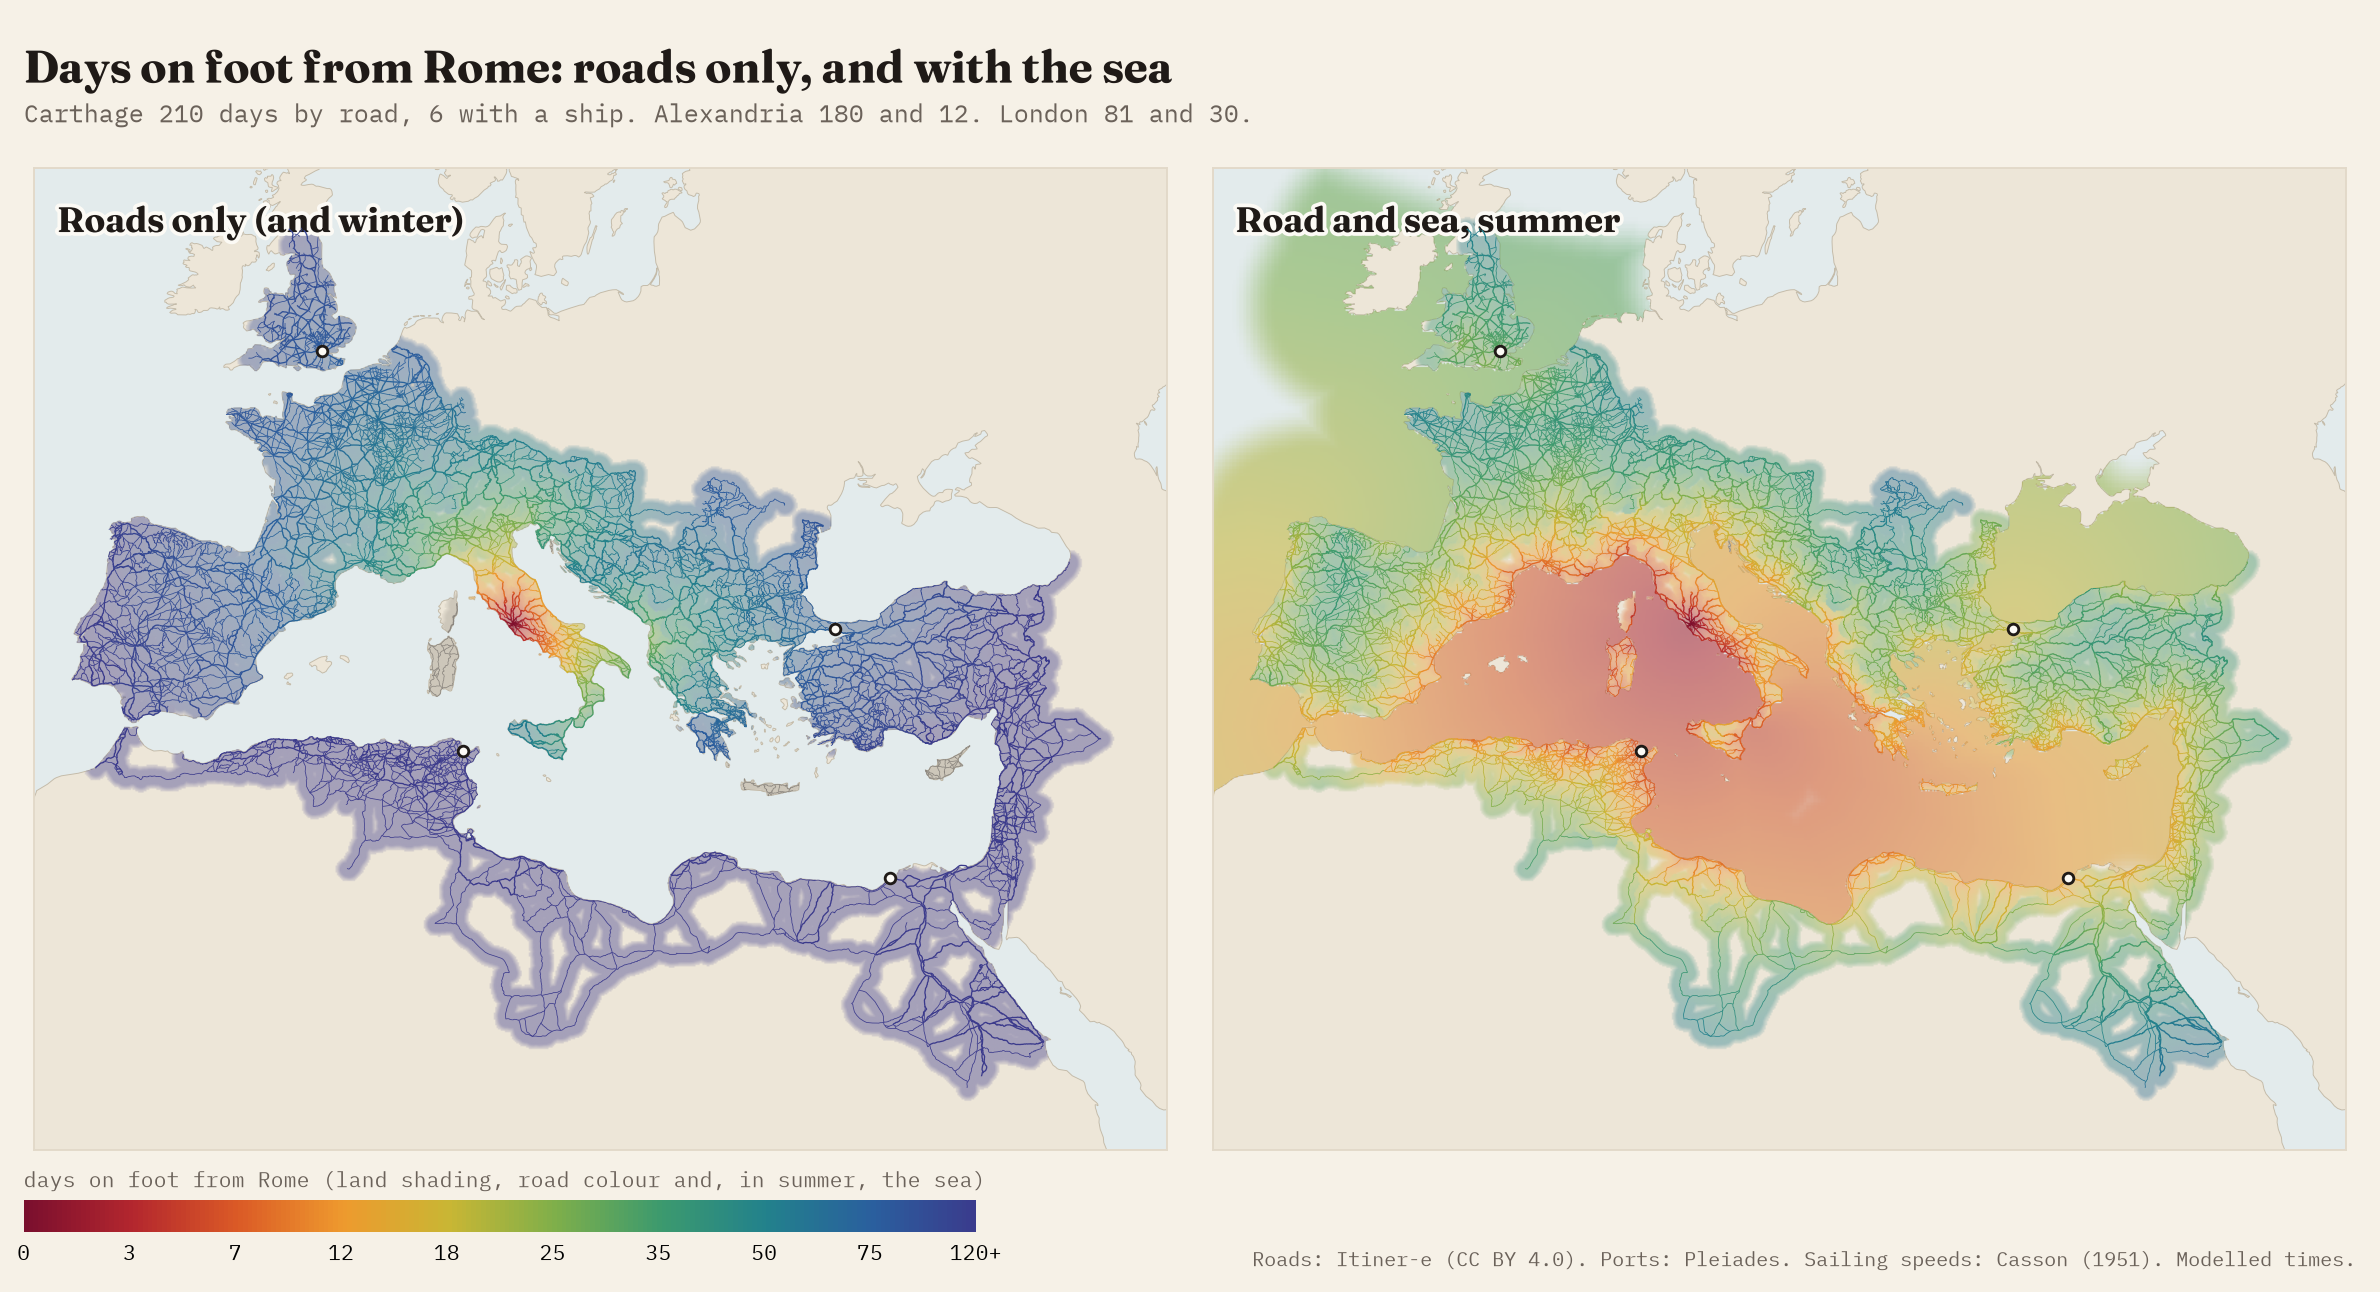
\includegraphics[width=\textwidth]{fig_side_by_side.png}\caption{Days on foot from Rome by road only (left) and by road and sea in summer (right). The sea shading shows the time to reach each sea cell.}\label{fig:side}\end{figure}

\begin{table}[tbp]\centering\small\caption{Modelled days from Rome: roads only (and winter) against road and sea in summer, on foot and by courier on land. Road and sea: model B. Range: the sensitivity tests, model A included. Model A: road and sea with Casson's median speeds. Port: where the ship is boarded.}\label{tab:cities}\begin{tabular}{lrrrrrrl}\toprule & \multicolumn{4}{c}{On foot} & \multicolumn{2}{c}{Courier} & \\ City & Road & Road and sea & Range & Model A & Road & Road and sea & Port\\\midrule
London & 81 & 29.9 & 28 to 35 & 32.4 & 23 & 20.3 & Portus (Trajan's harbour)\\
Constantinople (Istanbul) & 75 & 17.3 & 15 to 36 & 36.3 & 22 & 16.4 & Portus (Trajan's harbour)\\
Alexandria & 180 & 12.2 & 11 to 14 & 13.3 & 51 & 11.3 & Portus (Trajan's harbour)\\
Carthage & 210 & 5.8 & 5 to 8 & 6.2 & 60 & 4.9 & Portus (Trajan's harbour)\\
Antioch (Antakya) & 128 & 16.8 & 16 to 19 & 19.0 & 37 & 15.0 & Portus (Trajan's harbour)\\
Jerusalem & 157 & 17.3 & 16 to 20 & 18.8 & 45 & 14.3 & Portus (Trajan's harbour)\\
Cádiz & 116 & 13.3 & 12 to 16 & 14.5 & 33 & 12.5 & Portus (Trajan's harbour)\\
Marseille & 45 & 6.2 & 6 to 8 & 6.6 & 13 & 5.3 & Portus (Trajan's harbour)\\
Leptis Magna & 231 & 8.6 & 8 to 11 & 9.3 & 66 & 7.8 & Portus (Trajan's harbour)\\
Athens & 67 & 11.5 & 11 to 18 & 17.9 & 20 & 10.4 & Portus (Trajan's harbour)\\
York & 94 & 40.4 & 39 to 45 & 42.9 & 27 & 24.1 & Portus (Trajan's harbour)\\
Paris & 67 & 37.0 & 35 to 41 & 39.5 & 19 & 15.2 & Portus (Trajan's harbour)\\
\bottomrule\end{tabular}\end{table}

\begin{figure}[tbp]\centering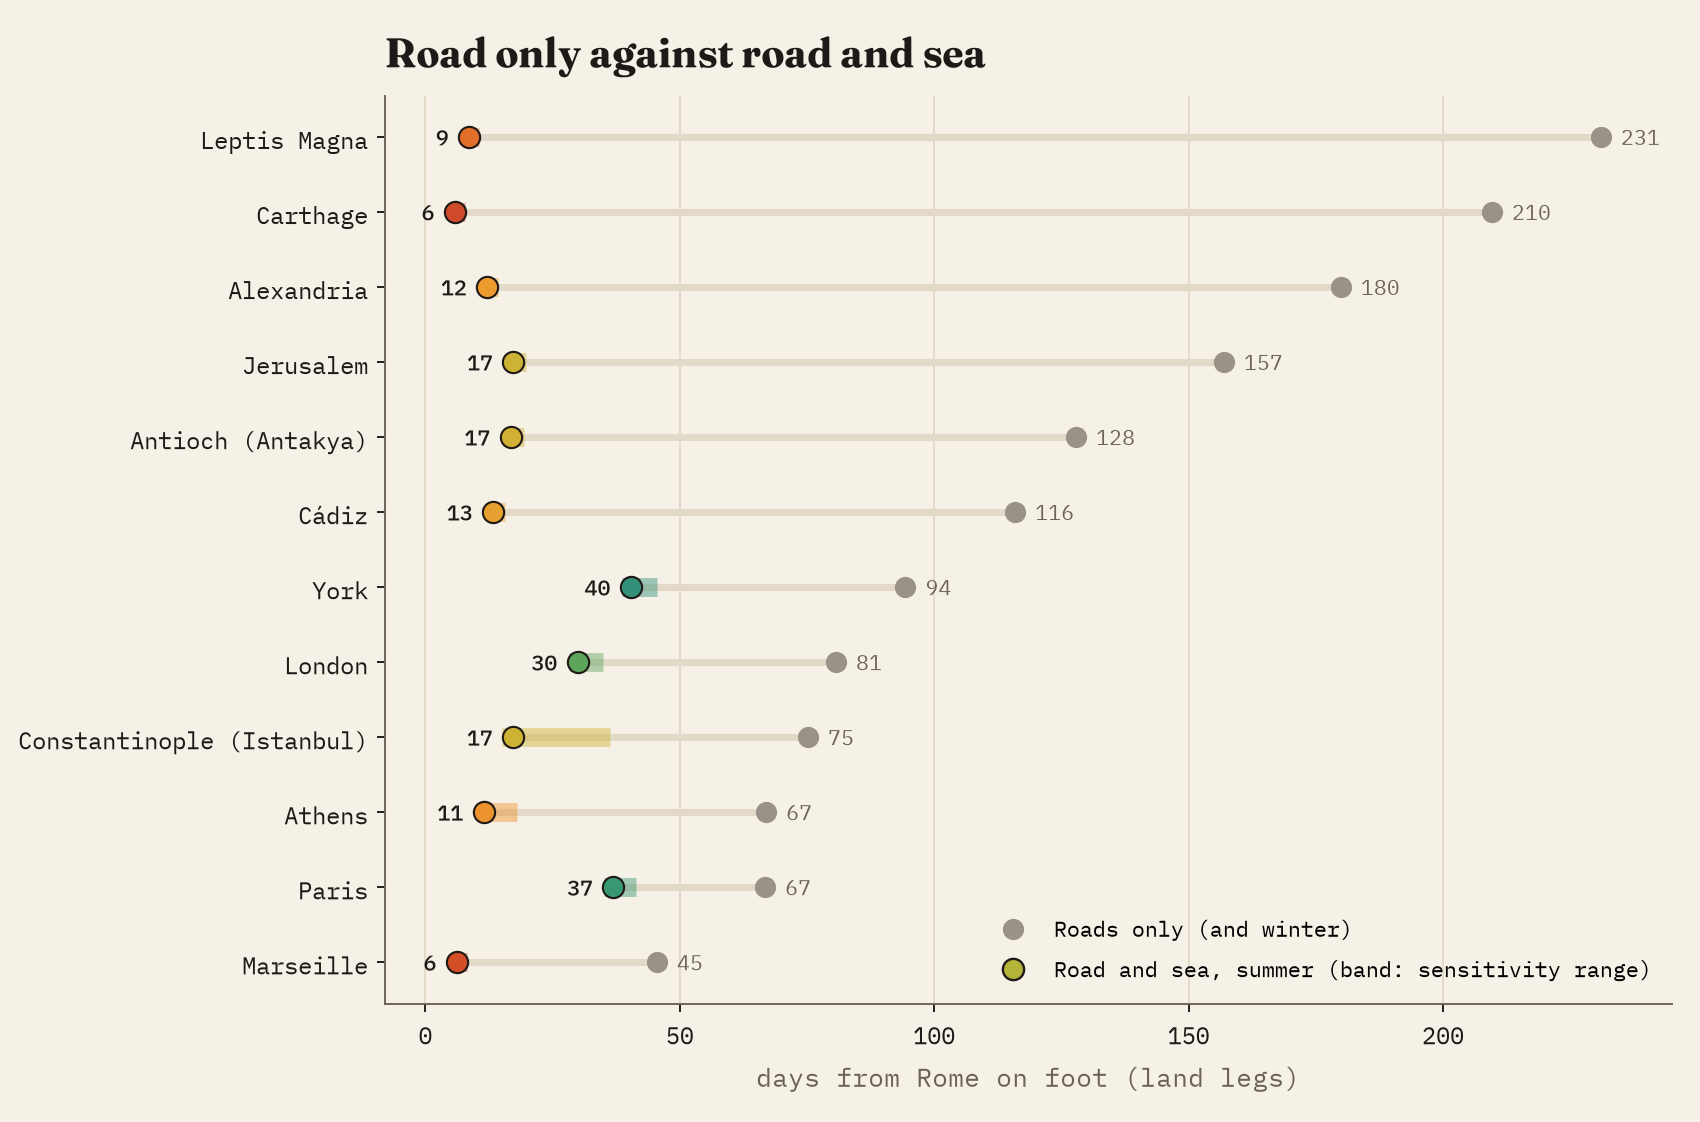
\includegraphics[width=.95\textwidth]{fig_cities.png}\caption{Days from Rome on foot: roads only (grey) and road and sea in summer (coloured), with the range from the sensitivity tests.}\label{fig:cities}\end{figure}

\subsection{How much of the empire was close}
By road alone, 0.5\% of the land of the provinces is within a week of Rome on foot, 1.4\% within a fortnight and 3.9\% within 30 days. With the sea in summer these become 1.2\%, 10.8\% and 59\% (Figure~\ref{fig:shares}). For a courier who rides the roads and takes ship where it helps, 92\% of the land is within 30 days. Measured on the road network instead of land area, the share of road length within 30 days on foot rises from 5.0\% to 65\%.

\begin{figure}[tbp]\centering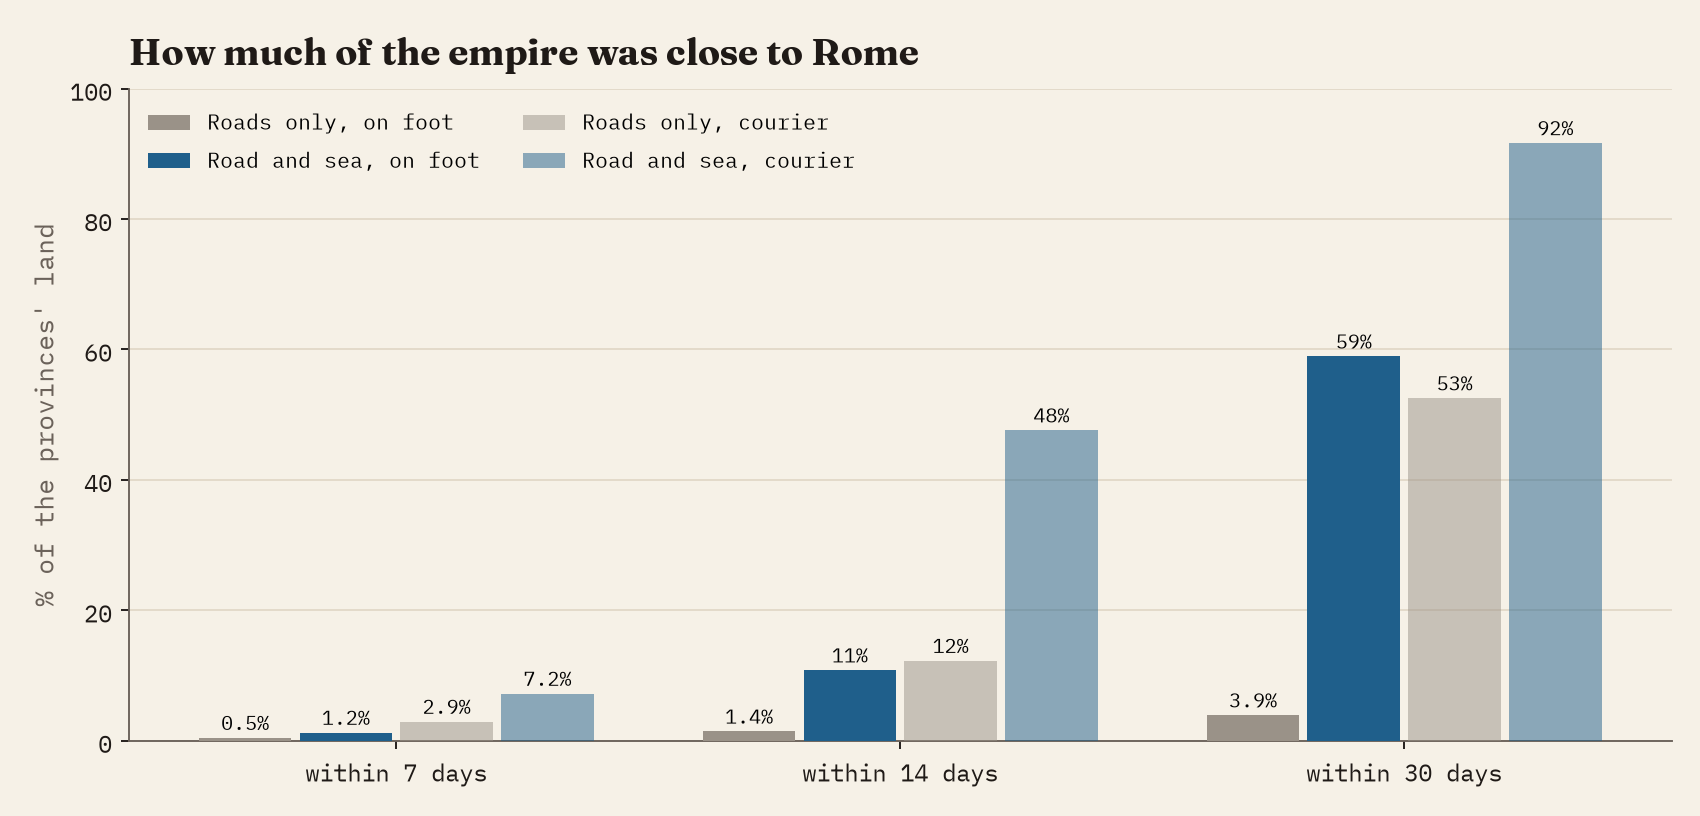
\includegraphics[width=.92\textwidth]{fig_shares.png}\caption{Share of the provinces' land (about AD 117) within 7, 14 and 30 days of Rome.}\label{fig:shares}\end{figure}

\subsection{Who gained most}
Of the 919 major ancient places in DARE that lie on the network, 94\% are reached more quickly in summer with the sea. Their median time from Rome on foot falls from 88 to 17 days. The largest gains are on the coast of Africa, which the roads reach only by going round (Table~\ref{tab:closest}): Carthage is 36.9 times closer, and the ports of Africa Proconsularis and Numidia 32 to 33 times. In absolute days the largest savings, over 200 days, are along the coast of Tripolitania and Cyrenaica. The 54 places that gain nothing are all in central Italy, within 14 days of Rome by road.

\begin{table}[tbp]\centering\small\caption{The major places the sea brought closest to Rome (days on foot; places at least 10 days from Rome by road).}\label{tab:closest}\begin{tabular}{llrrr}\toprule Place & Modern & Road & Road and sea & Times quicker\\\midrule
Carthago & Carthago & 210 & 5.7 & 36.9\\
Hadrumetum & Sousse & 211 & 6.4 & 33.1\\
Lepti Minus & Lamta & 212 & 6.5 & 32.8\\
Hippo Regius & Annaba & 199 & 6.3 & 31.7\\
Rusicade & Skikda & 195 & 6.5 & 29.8\\
Hippo Diarrhytus & Bizerte & 210 & 7.1 & 29.7\\
Uthina & Oudna & 209 & 7.6 & 27.5\\
Oea & Tripoli & 226 & 8.2 & 27.4\\
Sabratha & Sabratha & 223 & 8.2 & 27.1\\
Igilgili & Djidjelli & 190 & 7.0 & 26.9\\
\bottomrule\end{tabular}\end{table}

\subsection{Validation, and which model to headline}\label{sec:val}
Table~\ref{tab:models} and Figure~\ref{fig:val} compare the two models with Casson. Against his Table 1, model B falls inside his range for 14 of 57 passages (25\%) and near it for 36 (63\%), with a median of 1.01 times the middle of his range. Model A falls inside for 12 (21\%) and near for 25 (44\%), with a median of 1.38: it is systematically slow, and badly so on any passage with a northward leg in the Aegean or the Levant, because one speed into the wind has to serve both the long return from Alexandria and much shorter passages. On the 34 recorded voyages, model B's median is 1.01 times the reported time (1.10 for favourable passages and 0.90 for unfavourable ones), with 68\% of voyages within a factor of 1.5; model A's median is 1.49 (1.33 favourable, 3.01 unfavourable).

Model B has one clear failure. On the 4 long westward voyages home from the east (Alexandria to Rome, Naples and Massilia, and Rhodes to Rome) its median is 0.46 times Casson's estimate: Alexandria to Rome takes 30.2 days against his 53 to 73. Model A, fitted to that voyage, gets 3 of the 4 inside his range. No single pair of speeds into the wind reproduces both these voyages and the shorter passages of Table 1, which suggests that the long returns were slowed by more than the wind direction this model represents: waiting for a wind, coasting, calms and stops.

I headline model B for three reasons. It fits Casson's estimates far better overall; its speeds are all inside his stated ranges, so the calibration does not push any speed beyond what he regarded as plausible; and this study measures journeys from Rome, which run mostly with the summer wind, where model B matches him (Ostia to Alexandria in 11.0 days, inside his 10 to 13). The cost is that journeys ending in Italy from the east, which the interactive map can also compute, are too quick. Model A's answer is shown alongside every headline city in Table~\ref{tab:cities} and in the sensitivity ranges.

\begin{table}[tbp]\centering\small\caption{The two sea models: speeds (knots) and fit to Casson (1951). Inside: the model's time is within Casson's range; near: within a quarter of it. Ratios are model time over the middle of his range (Table 1) or over the reported time (voyages).}\label{tab:models}\begin{tabular}{lrr}\toprule & Model A (medians) & Model B (calibrated)\\\midrule
Downwind speed & 4.7 & 5.2\\
No prevailing wind & 3.35 & 3.7\\
Into the wind, central basin & 0.37 & 1.0\\
Into the wind, Aegean and Levant & 0.37 & 1.6\\
Ostia to Alexandria (days; Casson 10 to 13) & 12.1 & 11.0\\
Alexandria to Ostia (days; Casson 53 to 73) & 63.0 & 30.2\\
\midrule
Table 1 passages inside his range (of 57) & 12 (21\%) & 14 (25\%)\\
Table 1 passages inside or near & 25 (44\%) & 36 (63\%)\\
Table 1 median ratio & 1.38 & 1.01\\
Table 1 long voyages home from the east (4), median ratio & 0.97 & 0.46\\
Recorded voyages (34), median ratio & 1.49 & 1.01\\
\bottomrule\end{tabular}\end{table}

\begin{figure}[tbp]\centering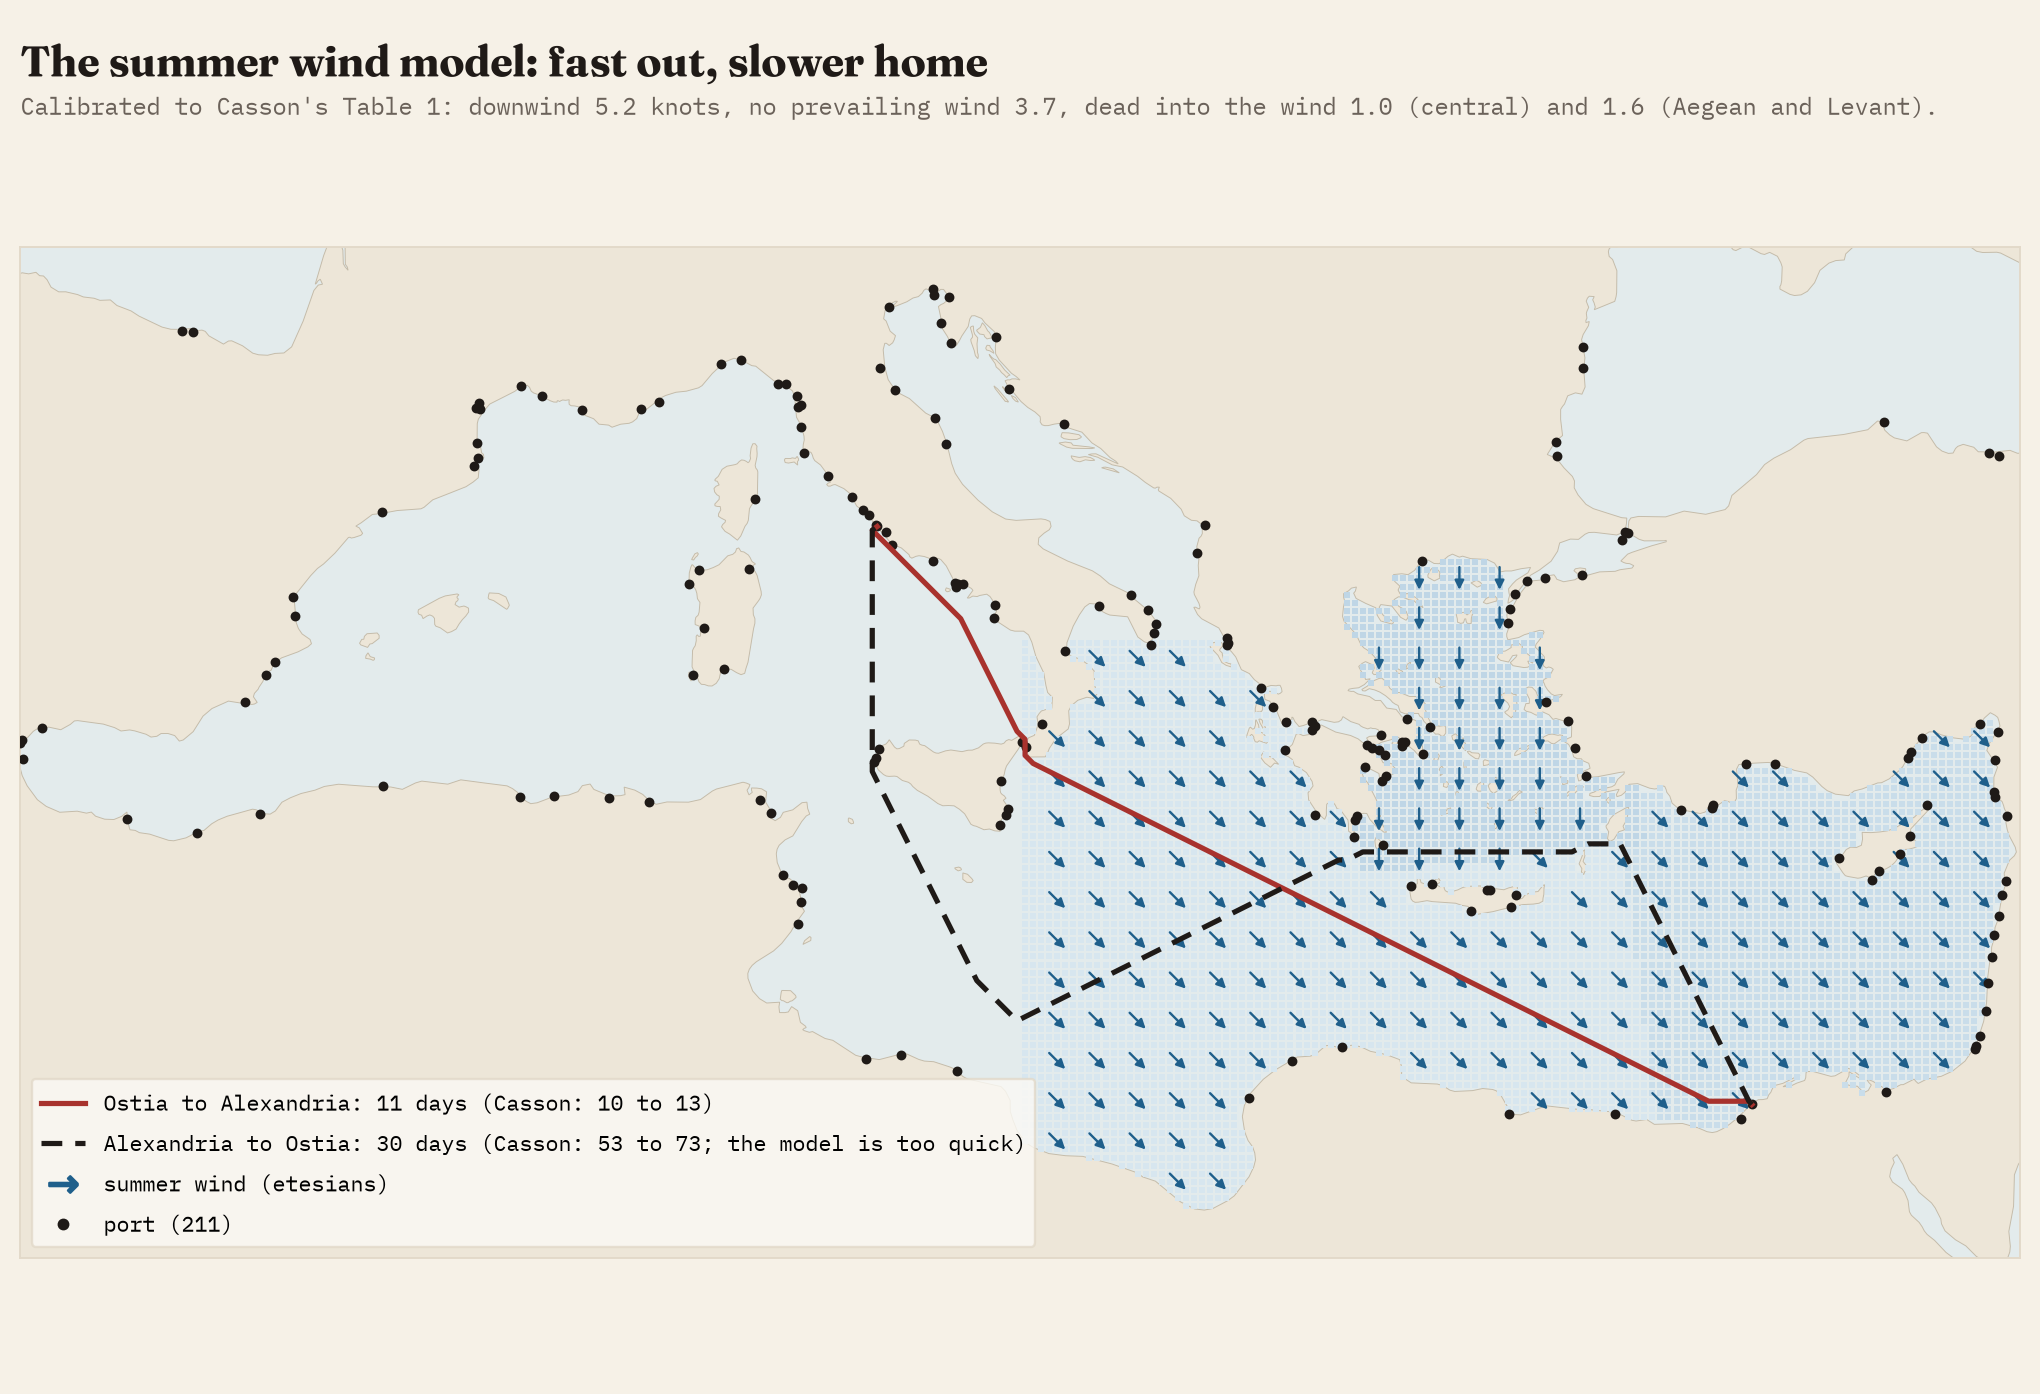
\includegraphics[width=\textwidth]{fig_wind.png}\caption{The summer wind model (model B): the wind basins (shaded), the direction the wind blows (arrows), the ports, and the model's routes from Ostia to Alexandria and back.}\label{fig:wind}\end{figure}

\begin{figure}[tbp]\centering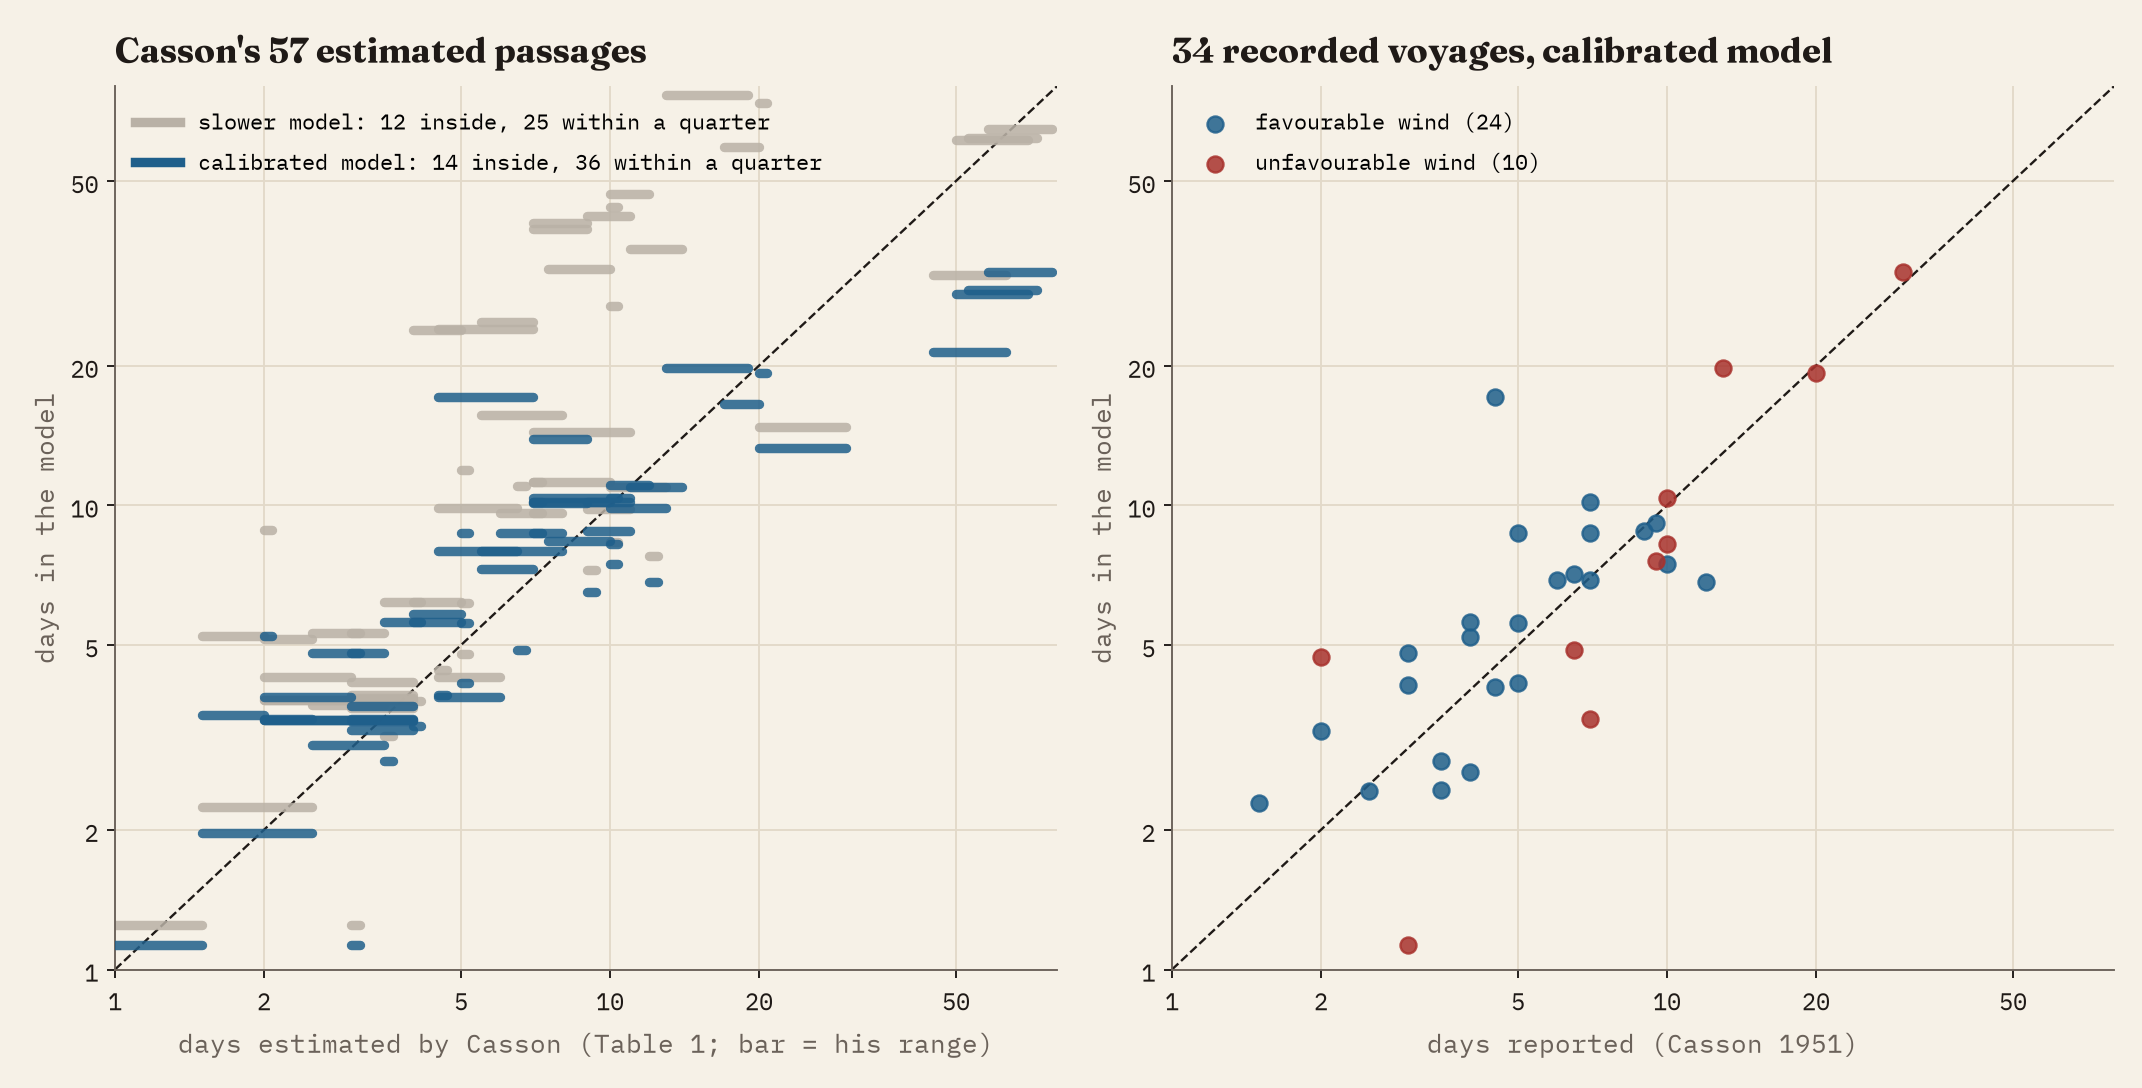
\includegraphics[width=\textwidth]{fig_validation.png}\caption{Left: the model's sea-only time for each passage in Casson's Table 1, drawn as a bar across his range of days at the height of the model's time, for model B (blue) and model A (grey). Right: model B against the recorded voyages in his other tables. Log scales.}\label{fig:val}\end{figure}

\subsection{Sensitivity}
Over all four sensitivity tests, model A included, the summer time on foot ranges from 5.3 to 7.8 days for Carthage, 11.4 to 14.3 for Alexandria, 28 to 35 for London and 15 to 36 for Constantinople. None changes the main contrasts; Constantinople, whose range comes almost entirely from model A, is the most uncertain.

\section{Discussion}
The sea did not shrink the empire evenly. It brought the coasts of Africa, Spain, Egypt and the Levant within a few weeks of Rome, while central Italy gained nothing and places far inland gained only the part of the journey a ship could take. And the wind made the sea one-way: Egypt was close to Rome, but Rome was far from Egypt. This is the same broad picture that ORBIS draws with a far richer model of winds and seasons \citep{scheidel2014}; the contribution here is to show it on a detailed, openly licensed road network with every assumption stated and checkable.

\section{Limitations}
The model has one summer wind pattern and no calms, storms, currents, night stops or winter sailing. Speeds come from a small record of voyages, biased to fast passages, calibrated to Casson's estimates, which are themselves reconstructions; the calibrated model makes the long voyages home from the east about twice as quick as he estimates. Only named ports are used, and every port can reach every other. The Red Sea and the rivers are left out because I found no sailing or towing speeds for them that I could check. All times are modelled, not recorded.

\section*{Data availability}
Derived data (ports, travel times from Rome for every junction, major places, Casson's voyages and the validation, and the full results) and all code are at \url{https://github.com/Tristan-Hotham/roman-travel-times} and archived with this paper. Itiner-e is licensed CC BY 4.0, Pleiades CC BY 3.0 and DARE CC BY; the derived data, figures and text are shared under CC BY 4.0, and the code is MIT licensed.

\section*{AI statement}
I wrote the text, with drafting and editing assistance from Claude (Anthropic), which also helped prepare the analysis code. I reviewed and checked all text and results.

\begin{thebibliography}{99}
\bibitem[{\AA}hlfeldt(2026)]{dare} {\AA}hlfeldt, J. (2026) Digital Atlas of the Roman Empire (DARE). Via \url{https://github.com/klokantech/roman-empire}. CC BY.
\bibitem[Casson(1951)]{casson1951} Casson, L. (1951) Speed under sail of ancient ships. \emph{Transactions and Proceedings of the American Philological Association} 82, 136-148. Online edition: \url{https://penelope.uchicago.edu/Thayer/E/Journals/TAPA/82/Speed_under_Sail_of_Ancient_Ships*.html}
\bibitem[de Soto et al.(2025a)]{itinere} de Soto, P., Pa\v{z}out, A., Brughmans, T. et al. (2025) A high-resolution dataset of roads of the Roman Empire: Itiner-e static version 2024. Zenodo. \url{https://doi.org/10.5281/zenodo.17122148}. CC BY 4.0.
\bibitem[de Soto et al.(2025b)]{desoto2025} de Soto, P., Pa\v{z}out, A., Brughmans, T. et al. (2025) Itiner-e dataset of Roman roads. \emph{Scientific Data}. \url{https://doi.org/10.1038/s41597-025-06140-z}
\bibitem[Dijkstra(1959)]{dijkstra1959} Dijkstra, E.W. (1959) A note on two problems in connexion with graphs. \emph{Numerische Mathematik} 1, 269-271.
\bibitem[Hotham(2026)]{hotham2026} Hotham, T. (2026) Roads of the Roman Empire: certainty, density, straight runs and days from Rome in the Itiner-e network. Zenodo. \url{https://doi.org/10.5281/zenodo.23857866}
\bibitem[Natural Earth(2026)]{naturalearth} Natural Earth (2026) 1:10m and 1:50m vectors. Public domain. \url{https://www.naturalearthdata.com/}
\bibitem[Pleiades(2026)]{pleiades} Pleiades: a gazetteer of past places (2026). \url{https://pleiades.stoa.org/}; GIS tables from \url{https://github.com/isawnyu/pleiades.datasets}. CC BY 3.0.
\bibitem[Scheidel(2014)]{scheidel2014} Scheidel, W. (2014) The shape of the Roman world: modelling imperial connectivity. \emph{Journal of Roman Archaeology} 27, 7-32.
\bibitem[Scheidel(2015)]{scheidel2015} Scheidel, W. (2015) ORBIS: the Stanford geospatial network model of the Roman world. Princeton/Stanford Working Papers in Classics.
\bibitem[Scheidel and Meeks(2012)]{orbis} Scheidel, W. and Meeks, E. (2012) ORBIS: The Stanford Geospatial Network Model of the Roman World. \url{https://orbis.stanford.edu/}
\bibitem[Wikipedia(2026a)]{wikietesian} Wikipedia contributors (2026) Etesian. English Wikipedia, revision 1378184207. CC BY-SA 4.0.
\bibitem[Wikipedia(2026b)]{wikimare} Wikipedia contributors (2026) Mare clausum. English Wikipedia, revision 1343557417. CC BY-SA 4.0.
\end{thebibliography}
\end{document}
